\section{Performance}

The HTCC is one of the major CLAS12 systems used in experiments with the electron beam. The most important
aspects of the HTCC performance are that it provides good timing, high electron detection efficiency, high signal
strength, and a high rejection factor for charged pions. All these parameters are critical for the quality of the data
obtained in experiments since the detector, in combination with the forward calorimeter~\cite{ec-nim}, provides a
fast trigger signal for CLAS12. As shown in Section~\ref{htcc-sim-sec}, the MC prediction for the HTCC
detection efficiency for electrons is $\approx$100\%. Fig.~\ref{fig:RAFO_2GeV} shows the experimentally
measured electron detection efficiency for elastically scattered electrons at 2~GeV. The corresponding thresholds
applied were approximately 2.5 photoelectrons. Measurements were performed using a special procedure with a
random trigger that was not correlated with the HTCC~\cite{trigger-nim}. There were observed 27 events not
detected by the HTCC due to the applied threshold. As shown, the electron detection efficiency is $\eta$ =
(99$\pm$0.2)\%, which is in good agreement with the MC estimate. This result can be considered as a conservative
estimate due to the relatively high threshold used in the measurements. Moreover, inelastically scattered electrons
travel a longer distance in the radiator gas (by 10\% to 30\% depending on the scattering angle). For these electrons
the signal strength is higher, and therefore the detection efficiency is higher as compared with the efficiency for
elastically scattered electrons.   

\begin{figure}[!ht]
    \centering
    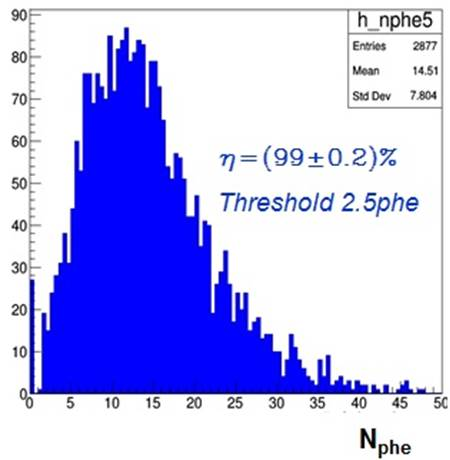
\includegraphics[width=1.0\linewidth,trim={0.0cm 0.0cm 0.0cm 0.0cm},clip]{images/RAFO_2GeV.jpg}
    \caption{Electron detection efficiency for elastically scattered electrons at 2~GeV. Data are obtained with the
      random trigger not correlated with the HTCC or other detector components of CLAS12.}
    \label{fig:RAFO_2GeV}
\end{figure}

Fig.~\ref{fig:positivePNPEC6595} shows the response of the detector over a wide range of particle momenta. The
increase in the number of events at high momentum ($>$5~GeV) is due to registration of charged pions (above
threshold for their registration in the HTCC) and this is clearly illustrated.

\begin{figure}[!ht]
    \centering
    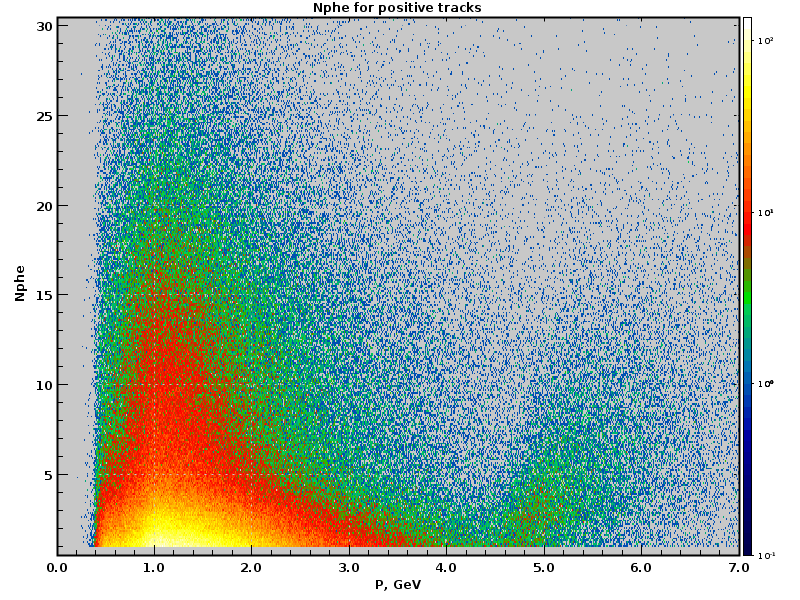
\includegraphics[width=1.0\linewidth,trim={0.0cm 0.0cm 0.0cm 0.0cm},clip]{images/positivePNPEC6595.png}
    \caption{Distribution of the HTCC response in terms of the number of photoelectrons vs. momentum over a wide
      momentum range, including the region beyond the threshold of charged pion registration ($>$5 ~GeV). Data were
      obtained for positrons and $\pi^+$-mesons.}
    \label{fig:positivePNPEC6595}
\end{figure}

%\begin{comment}
%  As shown bellow in the Fig.~\ref{fig:avgNPE_Theta_Phi_Dev_Build-2_NO_HOLES} the signal strength goes up for
%  the utmost mirrors (large electron scattering angles). This is because electrons travel a longer distance in the
%  radiator gas (10\% to 30\% difference depending on angle.) In other words the electron detection efficiency obtained
%  for elastically scattered electrons at 2 GeV can be considered as as a conservative estimate for the efficiency of
%  electron detection at larger angles.
%\end{comment} 

The signal strength in the HTCC depends on the actual properties of the mirror facets, such as their final shape
and reflectance. The accuracy of the combined mirror assembly and the alignment of the HTCC components (mirror,
PMTs, Winston Cones), and the composition of the radiator gas all influence the final results. The FADC histogram of
the typical signal strength distribution obtained in half-sectors \#1 and \#2 of sector~1 is shown in
Fig.~\ref{fig:Signal_S1_HS1_HS2_R1_R2}. The signal strength for scattered electrons averaged over all HTCC
channels is shown in Fig.~\ref{fig:Average_HTCC_Signal}. The experimentally measured mean value of 16.3
photoelectrons is close to the Monte Carlo simulation results, (see Fig.~\ref{fig:10cm_Targ_5T_Field_Phi}).

\begin{figure}[!ht]
    \centering
    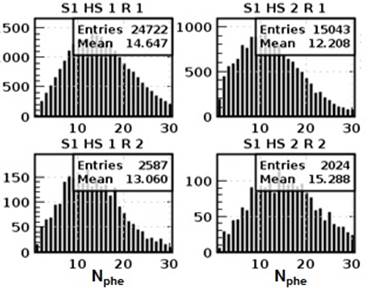
\includegraphics[width=1.0\linewidth,trim={0.0cm 0.0cm 0.0cm 0.0cm},clip]{images/Signal_S1_HS1_HS2_R1_R2.jpg}
    \caption{Typical distributions of the signal strength in channels covering polar angles in the range of $5^\circ$ to
      $12.5^\circ$ (Ring 1) and $12.5^\circ$ to $20.0^\circ$ (Ring 2) within an azimuthal interval of $60^\circ$.}
    \label{fig:Signal_S1_HS1_HS2_R1_R2}
\end{figure}

\begin{figure}[!ht]
    \centering
    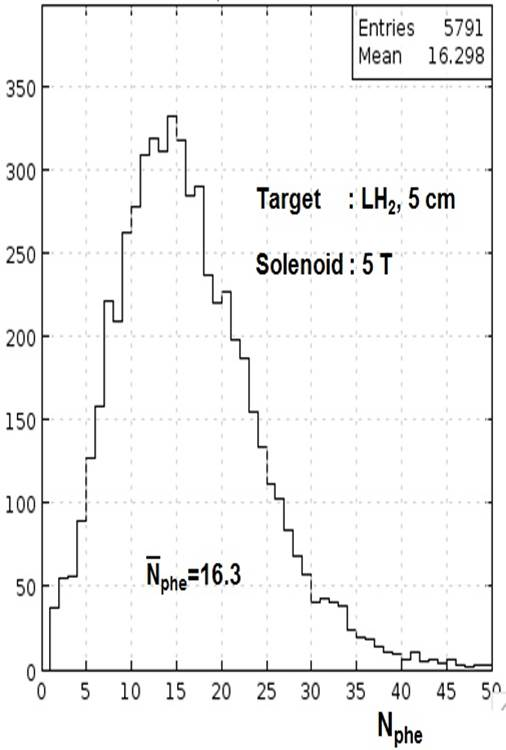
\includegraphics[width=1.0\linewidth,trim={0.0cm 0.0cm 0.0cm 0.0cm},clip]{images/Average_HTCC_Signal.jpg}
    \caption{The HTCC average signal strength for electrons from beam data at 10.6~GeV.}
    \label{fig:Average_HTCC_Signal}
\end{figure}

Fig.~\ref{fig:HTCC_Response_run4013} shows the HTCC response for different electron momenta.
Fig.~\ref{fig:avgNPE_Theta_Phi_Dev_Build-2_NO_HOLES}  shows the distribution of the HTCC response over
the entire face of the mirror in the $xy$ (transverse) plane. Similar distribution is shown in
Fig.~\ref{fig:avgNPE_XY_Dev_Build_02npe} obtained at a lower electron detection threshold of 0.2 photoelectrons.
The data shows that the integrated signal strength is about 16.5 photoelectrons. At large electron polar scattering
angles in range of 27.5$^\circ$ to 35$^\circ$, the statistics is lower.
Fig.~\ref{fig:statistics_Theta_Phi_Dev_Build_NO_HOLES} shows the distribution of statistics in all 6 sectors. 

\begin{figure}[!ht]
    \centering
    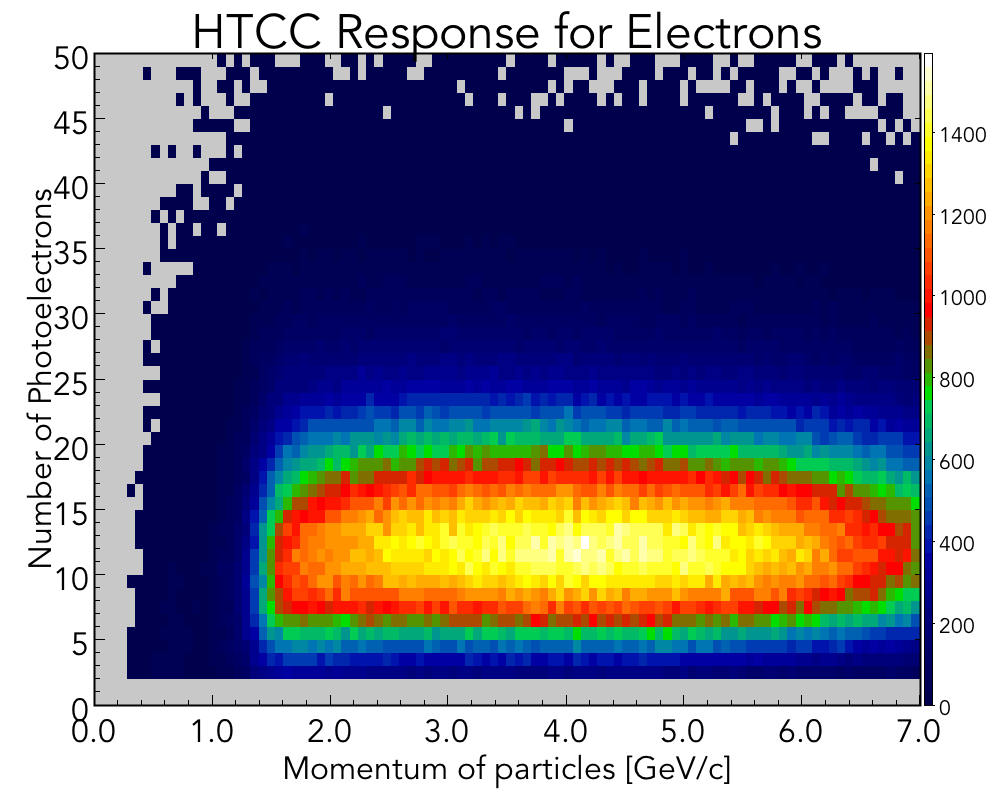
\includegraphics[width=1.0\linewidth,trim={0.0cm 0.0cm 0.0cm 1.73cm},clip]{images/HTCC_Response_run4013.png}
    \caption{The HTCC response for electrons: signal strength vs. momentum at 10.6~GeV energy.}
    \label{fig:HTCC_Response_run4013}
\end{figure}

\begin{figure}[!ht]
    \centering
    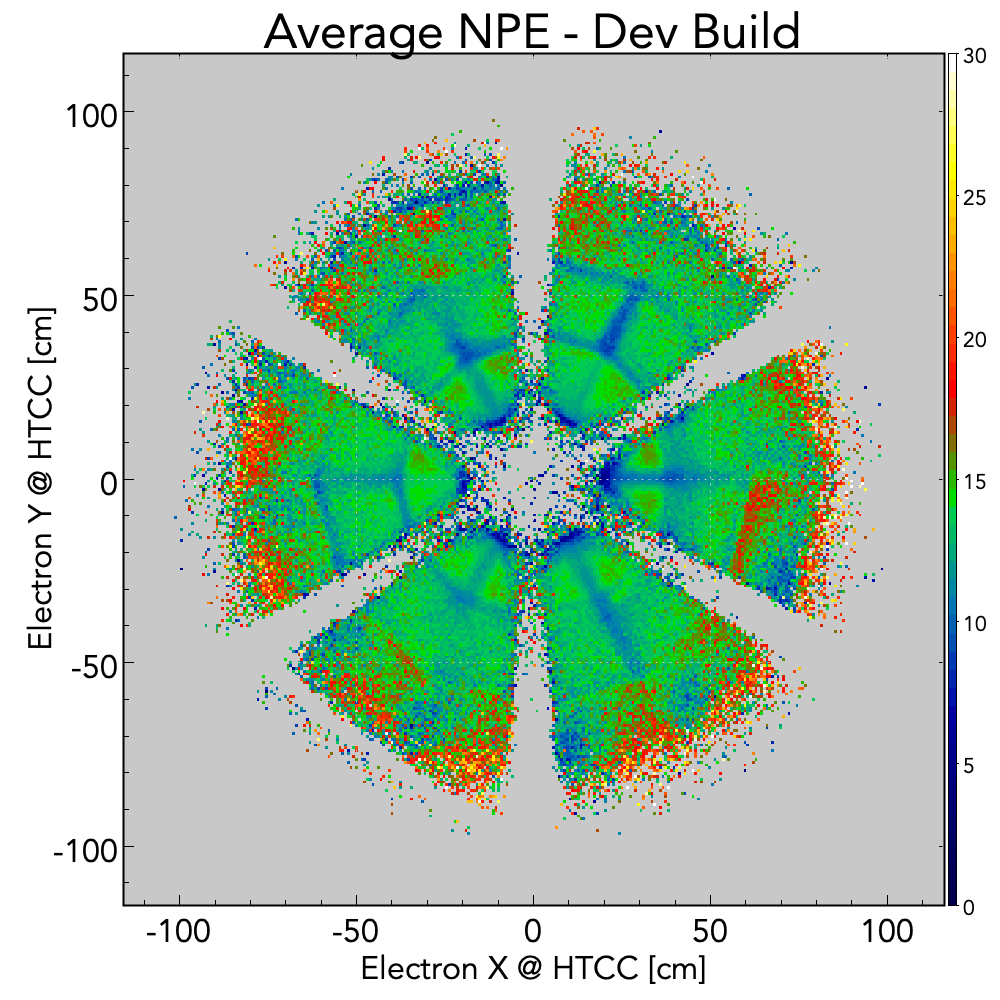
\includegraphics[width=1.0\linewidth,trim={0.0cm 0.0cm 0.0cm 1.67cm},clip]{images/avgNPE_Theta_Phi_Dev_Build-2_NO_HOLES.png}
    \caption{The HTCC response (in $N_{phe}$) for electrons in the $xy$-plane of the mirror.}
    \label{fig:avgNPE_Theta_Phi_Dev_Build-2_NO_HOLES}
\end{figure}

\begin{figure}[!ht]
    \centering
    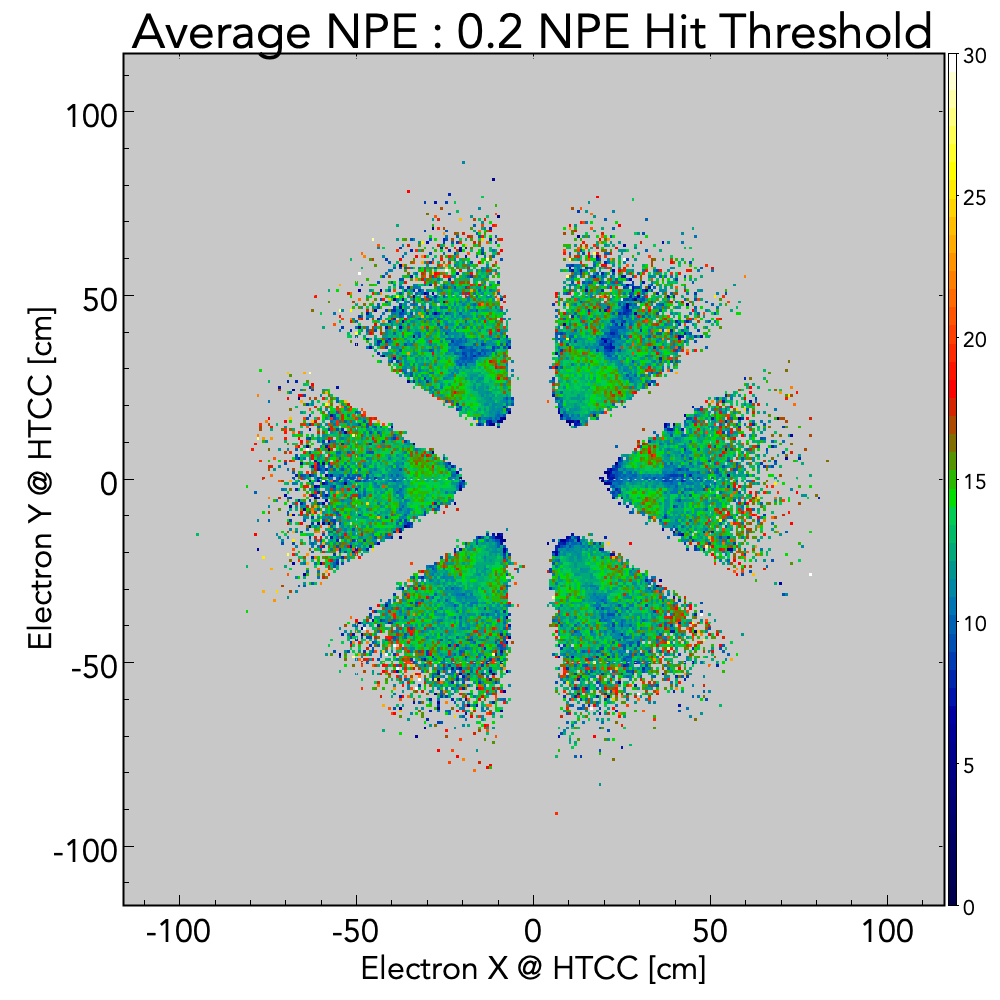
\includegraphics[width=1.0\linewidth,trim={0.0cm 0.0cm 0.0cm 1.67cm},clip]{images/avgNPE_XY_Dev_Build_02npe.png}
    \caption{The HTCC response (in $N_{phe}$) for electrons in $xy$-plane of the mirror at the electron detection
      threshold of 0.2 photoelectrons.}
    \label{fig:avgNPE_XY_Dev_Build_02npe}
\end{figure}

\begin{figure}[!ht]
    \centering
    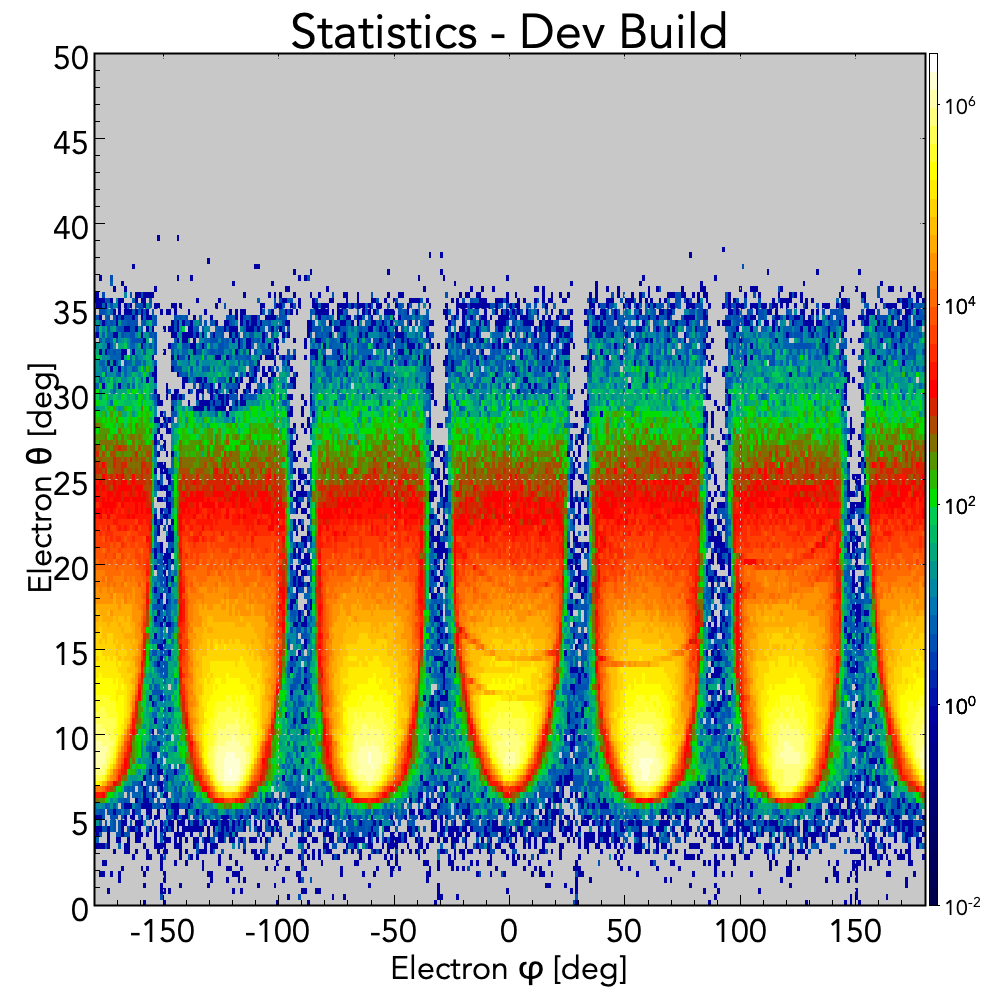
\includegraphics[width=1.0\linewidth,trim={0.0cm 0.0cm 0.0cm 1.67cm},clip]{images/statistics_Theta_Phi_Dev_Build_NO_HOLES.png}
    \caption{Distribution of statistics in all 6 sectors.}
    \label{fig:statistics_Theta_Phi_Dev_Build_NO_HOLES}
\end{figure}

We also note that in cases when the electrons cross a mirror close to its edges (at approximately at 5$^\circ$ and
35$^\circ$) one should expect unavoidable losses in the signal strength: some part of the Cherenkov light just passes
by the mirror. As far as the internal borders between adjacent mirrors are concerned, there are similar losses that
take place and are finally partially compensated due to the complete azimuthal symmetry of the detector, see
Fig.~\ref{fig:avgNPE_Theta_Phi_Dev_Build-2_NO_HOLES}. The width of the area along the internal boundaries that
is deformed in the direction normal to the mirror face due to the shrinkage of the glue is estimated to be between
$\sim 5 - 10$~mm. This area includes the technological zone of width $\sim$0.5~mm that does not reflect the light at
all. As a result these regions (width up to $\sim$10~mm) along the internal boundaries between the mirror facets
defuse the light impinging on the area, and therefore the signal strength is reduced. this edge effect is normal for
the given design of the detector.
